\documentclass{article}
\usepackage{amsmath}
\usepackage{graphicx}
\usepackage{bm}
\usepackage[margin=1in]{geometry}
\graphicspath{{images/}}
\begin{document}

\begin{center}
  A Tetrahedral Periodic Table
\end{center}

The periodic table of elements is one of the most recognizable scientific symbols in the world.

\begin{center}
  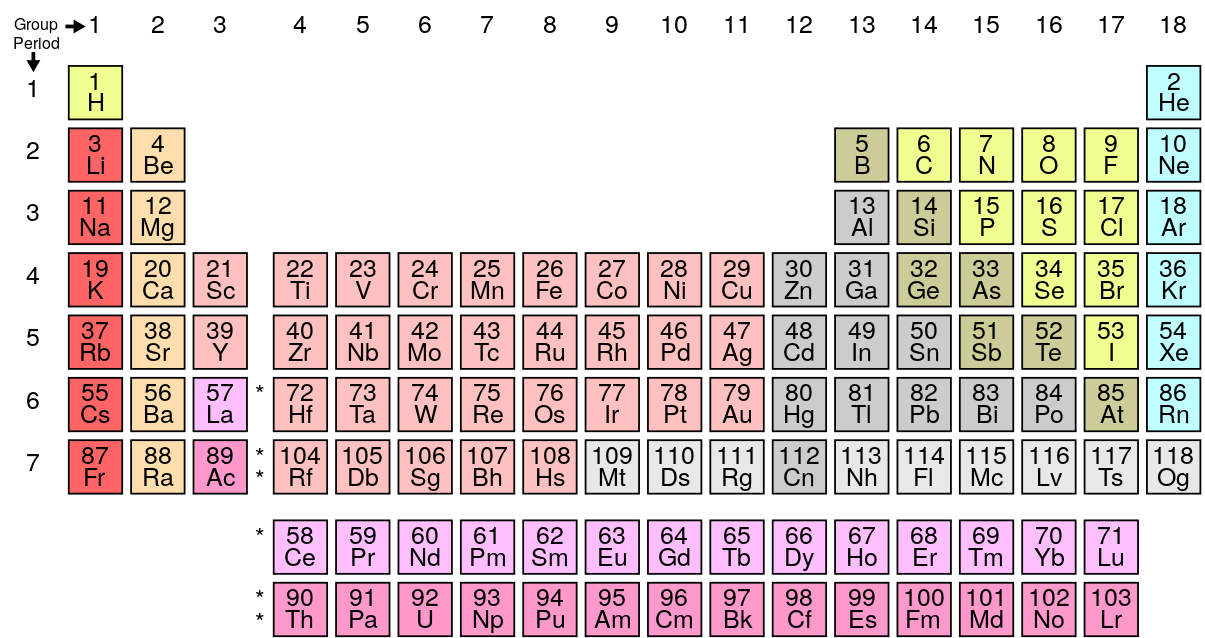
\includegraphics[width=\linewidth]{normal.png}
  \textit{Source: Offnfopt (Wikimedia Commons)}
\end{center}

The 118 known chemical elements are sorted into rows and columns,
where reading the table by rows yields the elements in order of atomic number
and the elements in a given column share chemical properties.
Each row terminates in a noble gas,
an atom whose outer electron shell is filled.
Since these shells grow in capacity in their filling order,
the rows of the table become progressively longer.
The row lengths, AKA periods, are 2, 8, 8, 18, 18, 32, and 32.
The last two rows are often, as above, interrupted
into two segments totaling 18 elements, which are placed with the rest of the table,
and a segment of 14, which is placed below it.
(These segments of 14 are the lanthanides and actinides.)
Without interruption, the table looks as follows.

\begin{center}
  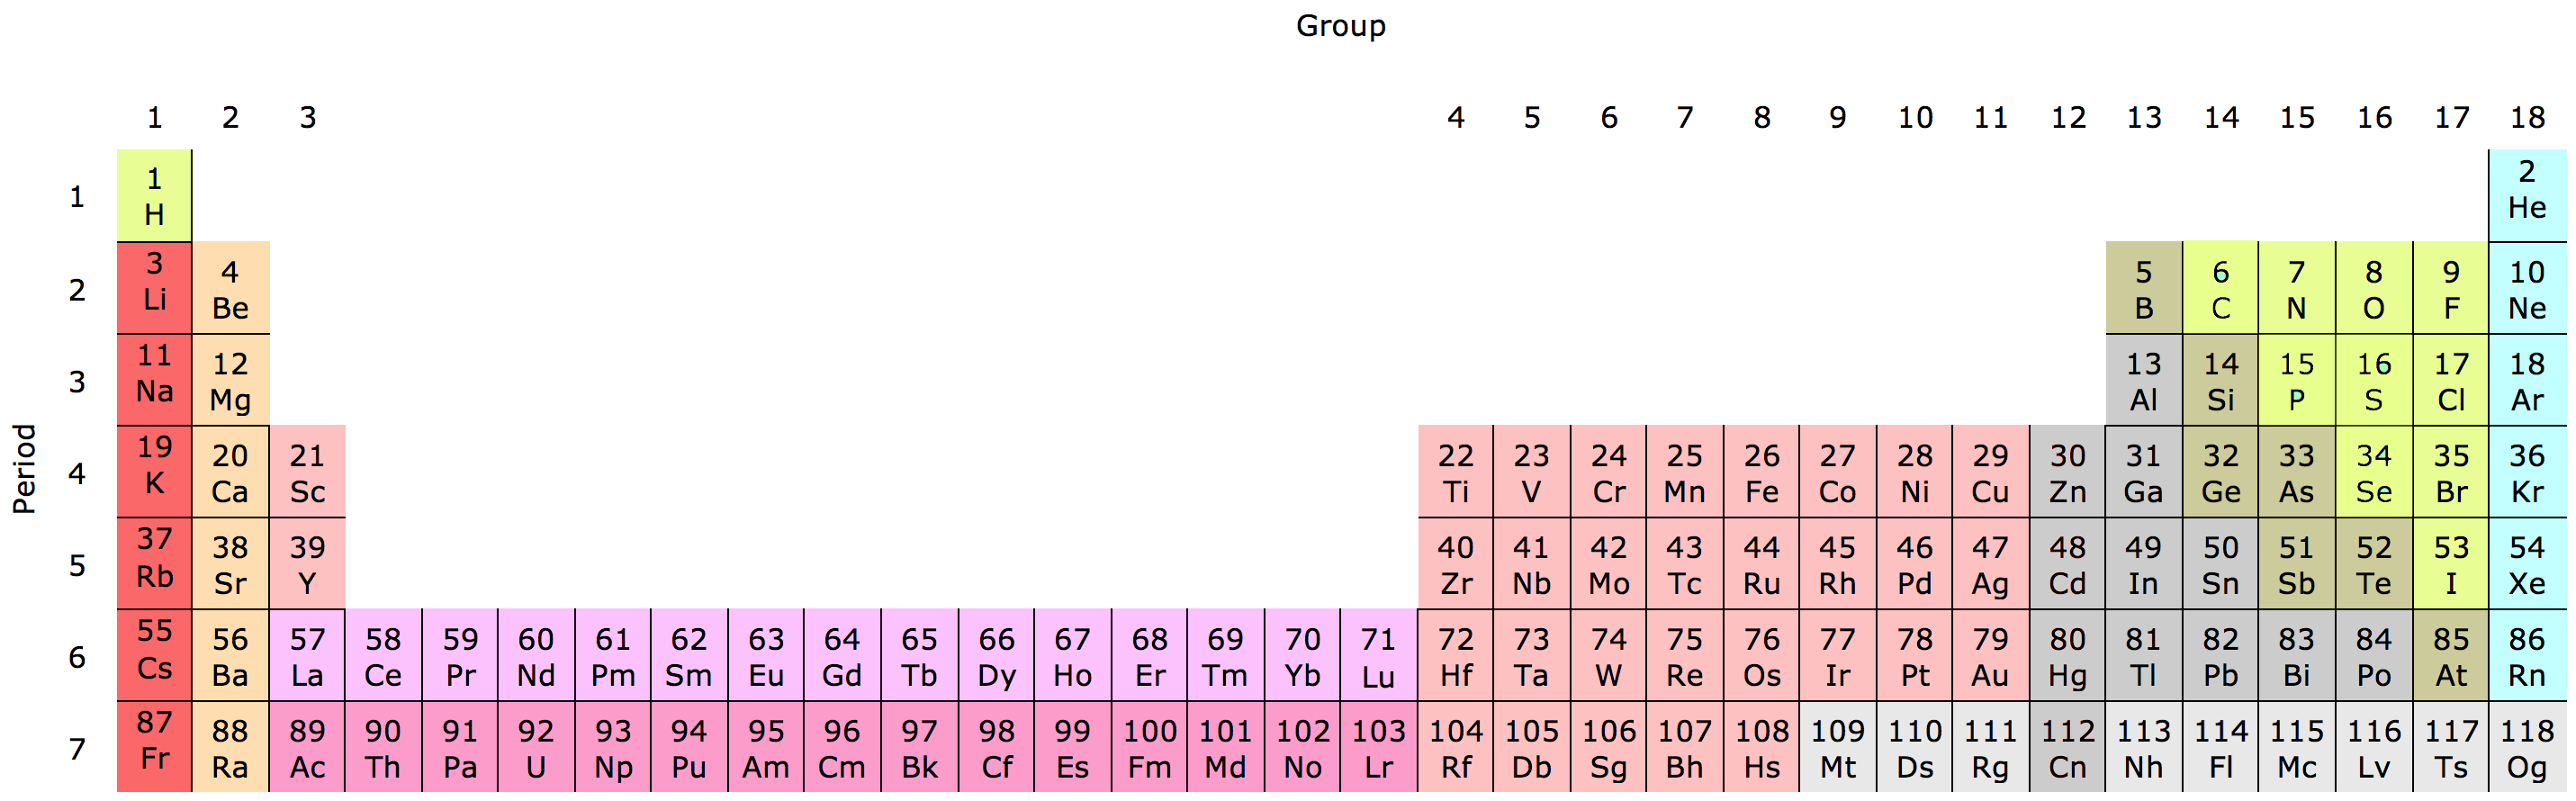
\includegraphics[width=\linewidth]{long.png}
  \center{\textit{Source: Sandbh (Wikimedia Commons)}}
\end{center}

But, where do the period lengths come from?


The answer has to do with the solutions to the Schr{\"o}dinger equation,
which are described by the four quantum numbers (QNs).
Each quadruplet of QNs represents a potential state of an electron orbiting the nucleus.
The numbers and their constraints are as follows:

\begin{center}
  \begin{tabular}{|c c c c|}
    \hline
    Name & Variable & Constraints & \# of values \\
    \hline
    Principal QN & $n$ & Integer, $0 < n$ & $\infty$ \\
    Azimuthal QN & $\ell$ & Integer, $0 \leq \ell < n$ &  $n$ \\
    Magnetic QN & $m_\ell$ & Arbitrary & $2\ell+1$ \\
    Spin QN & $m_s$ & Arbitrary & 2 \\
    \hline
  \end{tabular}
\end{center}

A pair of $n$ and $\ell$ describes a subshell of electrons,
and $m_\ell$ and $m_s$ index an electron within that subshell.
A subshell is written with $n$ followed by a letter based on $\ell$:

\begin{center}
  \begin{tabular}{|c|c c c c|}
    \hline
    $\ell$ & 0 & 1 & 2 & 3 \\
    Letter & s & p & d & f \\
    \hline
  \end{tabular}
\end{center}

For example, the subshell where $n=2$ and $\ell=1$ would be written ``2p.''
The potential subshells as given by the constraints are as follows:

\begin{center}
  \begin{tabular}{|c|c c c c c|}
    \hline
    n,$\ell$ & 0 & 1 & 2 & 3 & \ldots \\
    \hline
    1 & 1s & & & & \\
    2 & 2s & 2p & & & \\
    3 &3s & 3p & 3d & & \\
    4 & 4s & 4p & 4d & 4f & \\
    \vdots & \vdots & \vdots & \vdots & \vdots & $\ddots$ \\
    \hline
  \end{tabular}
\end{center}

Note that the latter two QNs are arbitrary,
i.e. only the number of possible solutions matters.
Their usual values are
$-\ell \leq m_\ell \leq \ell$,
$m_s = \pm \frac{1}{2}$.
The periodic table proposed here, however, will use
$0 \leq m_\ell \leq 2\ell$ and $m_s = 0$ or $1$,
for reasons that will become clear later.

Starting from hydrogen,
each element has one more proton than the last,
so each also has one more electron, assuming the atoms are neutral.
An atom attempts to minimize the total energy of its electrons,
so in general, the sequence of electrons added as the atomic number increases
is ordered from least to greatest energy.

The sentence is complete.

\begin{enumerate}
\item $n+\ell$, increasing
\item $\ell$, decreasing
\item $m_s$, arbitrary
\item $m_\ell$, arbitrary
\end{enumerate}

\begin{enumerate}
\item $n+\ell$, increasing, front $\rightarrow$ back (Madelung rule)
\item $2\ell+m_s$, decreasing, left $\rightarrow$ right (Hund's rule)
\item $m_\ell$, arbitrary, bottom $\rightarrow$ top
\end{enumerate}

\newpage

h

\end{document}
